\chapter{\label{ch:1-intro}Introduction} 

%\minitoc

\section{Overview}
...

% 1
\section{The adaptive immune system}
Humans are exposed to millions of potential pathogens every day and therefore require defences to be able to protect themselves against infection.
These defences can be innate or adaptive.
An example of an innate defence is the skin acting as a physical barrier between the outside world and the body.
Another example of an innate defence is non-specific engulfing (phagocytosis) of foreign pathogens by macrophages (a type of white blood cell).
Innate responses are relied upon as the first line of defence, however sometimes a more sophisticated, specialised response is required- called the adaptive immune response. (REF-mol biology of the cell).

Adaptive immune responses are specific to the pathogen that induced the response and are dependent on B cells and T cells, two major classes of lymphocytes (a class of white blood cell).
Two classes of adaptive immune responses exist: antibody responses, co-ordinated by B cells, and cell mediated immune responses, co-ordinated by T cells.
T-cell-mediated immune responses recognise foreign antigens (antibody generators;
substances capable of eliciting an immune response by stimulating B or T cell activation) on the surface of cells and can either kill the pathogen-infected cells or stimulate B cells or phagocytes to help eliminate the pathogen.
In antibody responses, B cells and plasma cells secrete antibodies, also known as immunoglobulins.
Immunoglobulins are large Y-shaped proteins, which recognise and bind to the specific foreign antigen on the pathogen which stimulated their production.
Binding of immunoglobulins to antigens renders the virus or microbial toxin inactive as it blocks their ability to bind to host cells.
Additionally, antibody binding makes it easier for phagocytic cells to ingest the pathogen.
%%%%%%


%2
\subsection{Plasma cells}
%3
\subsubsection{Plasma cell development}
Stem cells are precursor cells which can give rise to at least one type of differentiated (mature) cell, with the capability of indefinite self-renewal.
Hematopoietic stem cells (HSC) are stem cells that give rise to all the cells of the hematopoietic system.
Two predominant cell populations are produced by HSCs: the common myeloid progenitor (CMP) and the common lymphocyte progenitor (CLP).
CMP differentiation produces erythrocytes (red blood cells), mast cells, monocytes, macrophages, neutrophils, eosinophils, basophils and myeloid dendritic cells.
CLP differentiation results in B cells, T cells, natural killer (NK) cells and lymphoid dendritic cells.

%% Immune cell figure
\begin{figure}
\centering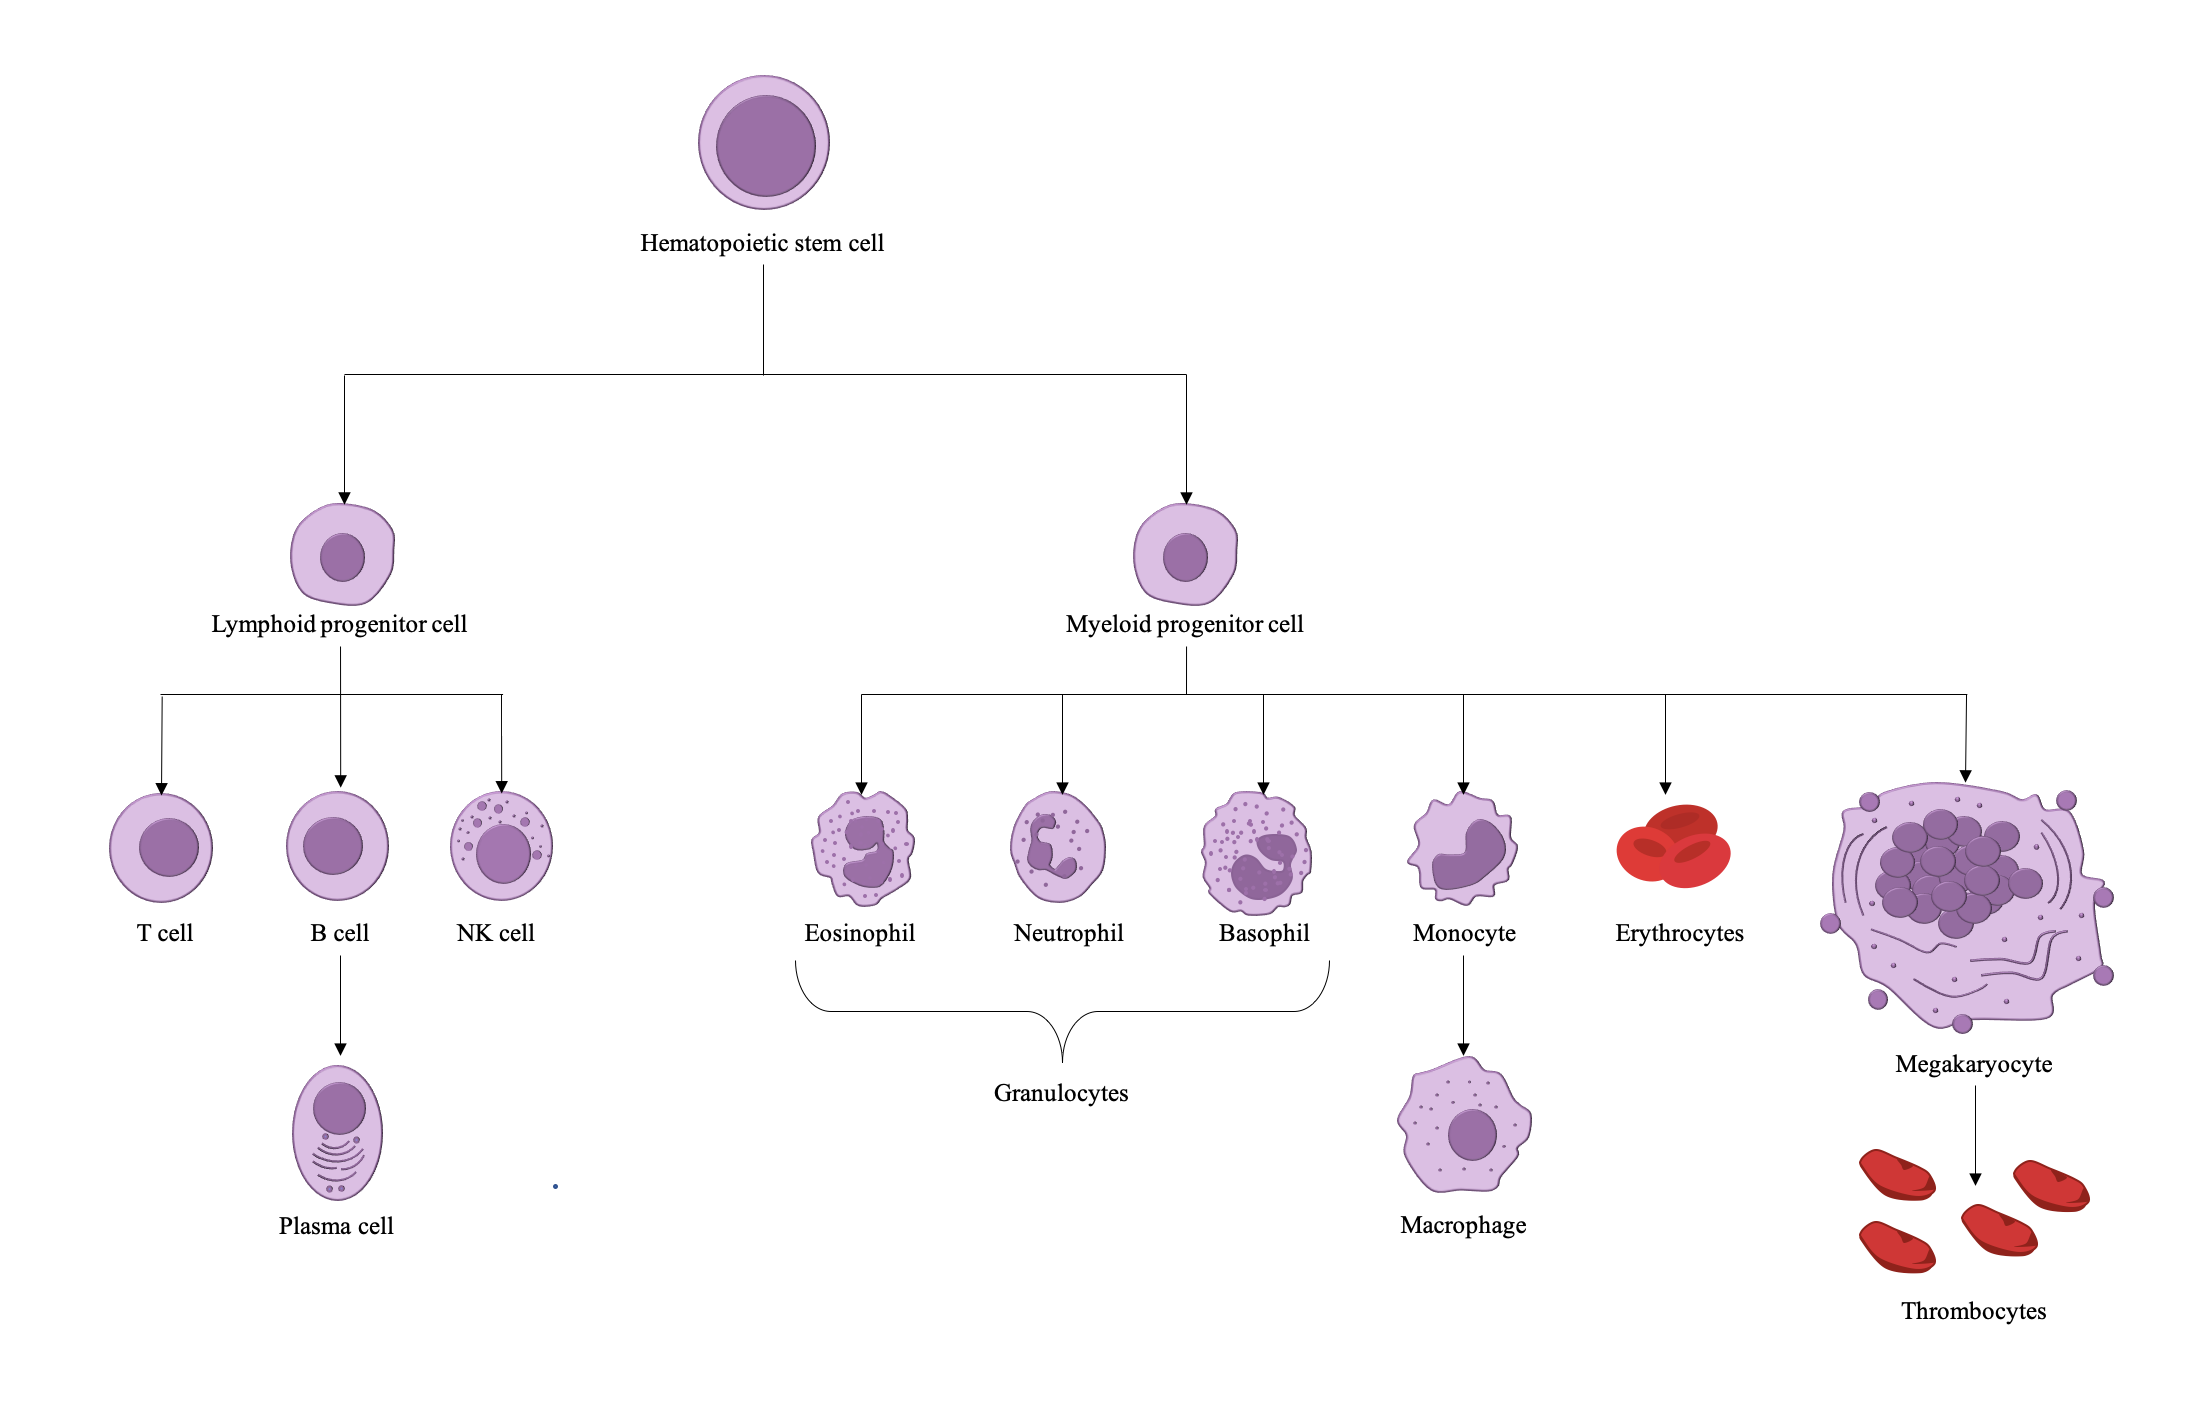
\includegraphics[width=0.7\textwidth]{figures/Introduction/immune_cells.png}
\caption[Hematopoietic system cell differentiation]{Hematopoietic stem cell (HSC) cell differentiation. HSCs divide into myeloid or lymphoid progenitor cells. Dendritic cells and a number of precursor states have been ommitted. }
\label{fig:HSC_differentiation}\end{figure}
%%

Most B cells die in the bone marrow soon after developing, however some will develop in the bone marrow, where initial stages of maturation occur and then migrate to secondary lymphoid organs, such as the spleen.
Within secondary lymphoid organs, numerous critical decisions on B cell fate are made, involving complex transcriptional networks, cell interactions, gene rearrangements, and mutations\cite{roth2014tracking, jourdan2011characterization}.
Upon antigenic-stimulation, naive B cells differentiate into memory B cells or plasma cells.
Terminally differentiated plasma cells are the final effectors of the B cell lineage, each dedicated to secreting large amounts of a single type of antibody.
Plasma cells have an extensive rough endoplasmic reticulum (ER), and have numerous genes involved in immunoglobulin secretion upregulated, including \textit{XBP-1} and \textit{CHOP}\cite{shapiro2004plasma}, to enable the production of copious amounts of antibody.
Plasma cells appear to consist of two distinct categories: short-lived plasma cells, which have life-spans of several months and are located in extrafollicular locales such as in medullary chords of lymph nodes or the red pulp of the spleen, and long-lived plasma cells, which have life-spans of decades and are mainly found in the bone marrow\cite{bortnick2013and, andraud2012living}.



%1
\section{Multiple myeloma}
%2
\subsection{Multiple myeloma cells}
Multiple myeloma is a malignancy of terminally differentiated plasma cells.
It is characterised by aberrant proliferation of clonal, long-lived plasma cells in the bone marrow\cite{anderson2011pathogenesis}.

%2
\subsection{Epidemiology}
Multiple myeloma accounts for 1-2\% of all cancers and has the second highest incidence of hematological malignancies, after non-Hodgkin's lymphoma\cite{international2003criteria}.
MM is rare in individuals under the age of 40, with the average age at time of diagnosis centering around 70\cite{tsang2019multiple, palumbo2011multiple}.
MM is more prevalent in males than females and is around twice as common in black populations than in Caucasian or Asian populations\cite{nhsmyeloma}.
The average incidence rate is approximately 1-6 cases per 100000 individuals\cite{tsang2019multiple, palumbo2011multiple, teras20162016}, with the highest age-standardised incidence rates in the regions of Australasia, North America, and Western Europe\cite{cowan2018global}.
Five-year survival rate of MM patients is approximately 49\%, whilst approximately a third of MM patients survive ten years or greater\cite{cancerresearchuk, siegel2016cancer}.
%While there have been many successful medicines developed for myeloma, they all suffer from the development of drug resistance.

%2
\subsection{Presentation}
%3
\subsubsection{Precursor states}
All cases of MM are preceded by asymptomatic precursor states, monoclonal gammopathy of unknown significance (MGUS) and smoldering multiple myeloma (SMM).
However, only some patients with SMM or MGUS progress to active MM.

MGUS is a pre-malignant condition where patients have the presence of monoclonal immunoglobulins in their blood or urine, $<$10\% clonal plasma cells in their bone marrow, but lack any myeloma-related end-organ damage\cite{van2018mgus}.
Patients with SMM have between 10 and 60\% clonal plasma cells in their bone marrow, serum monoclonal immunoglobulin of $\ge$3 g/dL, and like MGUS, have no signs of end-organ damage\cite{rajkumar2015smoldering}.
Progression risk of MGUS into symptomatic MM is about 1\% per year, whilst progression risk of SMM to MM is higher, at around 10\% per year for the first 5 years, after which it decreases\cite{korde2011monoclonal, kyle2007clinical}.
%

%3
\subsubsection{Active MM}
There are multiple classifications of active MM.
The International Myeloma Working Group's definition\cite{rajkumar2014international} is as follows:
Greater than 10\% clonal plasma cells located in the bone marrow and one or more myeloma-defining event or biomarker of malignancy.
Myeloma defining events consist of evidence of end-organ damage that can be attributed to the surplus of M protein and clonal plasma cells, namely the CRAB features:
%
% List of myeloma events (CRAB)
\begin{itemize}
  \item Hypercalcemia
    \begin{itemize}
        \item Serum calcium $>$ 1 mg/dL higher than the upper limit of normal, or
        \item Serum calcium $>$ 11 mg/dL
    \end{itemize}
  \item Renal insufficiency
    \begin{itemize}
        \item Creatinine clearance $<$ 40 mL per min, or
        \item Serum creatine $>$ 2 mg/dL
  \end{itemize}
  \item Anemia
    \begin{itemize}
        \item Hemoglobin value of $>$  20 g/L below the lower limit of normal, or
        \item Hemoglobin value $<$ 100 g/L
    \end{itemize}
    \item Bone lesions
      \begin{itemize}
        \item One or more osteolytic lesions on skeletal radiography, CT or PET-CT
        \end{itemize}
\end{itemize}
% End of list
%

Biomarkers of malignancy include greater than or equalt to 60\% clonal plasma cells in the bone marrow, an involved:uninvolved serum free light chain ratio greater than or equal to 100, and more than one focal lesion on an MRI study\cite{rajkumar2014international}.

%
It is currently unclear what causes the malignant transformation between precursor states and active MM\@.
However certain factors have been identified as risk factors, including point mutations, a large array of up-regulated transcription factors, and numerous immune events.

\subsection{Treatment of multiple myeloma}
Multiple myeloma may be an incurable disease, however it is treatable.
In fact, in the last decade median survival time for newly diagnosed MM patients has almost doubled\cite{kazandjian2016look}.
Novel therapeutic advances have contributed to this improvement (Table\ref{tab:treatment_history}).

% Timeline of treatment options
%% Table for treatment timeline


\begin{table}[h]
\centering
\begin{tabular}{|p{1cm}|p{3cm}|p{8cm}|p{1.3cm}|}
\hline
\textbf{Year} & \textbf{Treatment} & \textbf{Usage} & \textbf{Ref} \\ \hline
1958 & Melphalan & The alkylating agent melphalan was first used in plasma cell myeloma in 1958. & \cite{blokhin1958clinical} \\ \hline
1960s & Corticosteroids & Placebo-controlled double-blind trial of prednisone in multiple myeloma. Combinations of prednisone and melphalan showed an increased survival over melphalan alone. Dexamethasone and prednisone have become a cornerstone in the treatment of multiple myeloma. & \cite{mass1962comparison, alexanian1969treatment} \\ \hline
1980s & Stem-cell transplantations & Numerous successful allogenic and autologous bone marrow transplantations in patients with multiple myeloma &  \cite{mcelwain1983high, osserman1982identical, fefer1986identical, gahrton1987bone}  \\ \hline
2003 & Proteasome inhibitors & Bortezomib, a first-in-class proteasome inhibitor, was first approved by the FDA for use in relapsed and refractory multiple myeloma. In 2008 it was approved for patients with no prior treatment. Carfilzomib was approved in 2012 for advanced MM and later in 2015 for treatment of relapsed MM. The oral proteasome inhibitor, ixazomib, was approved as a combination treatment with lenalidomide and dexamethasone in 2016 for people who have received at least one previous treatment. & \cite{kane2003velcade,richardson2003phase,katsnelson2012next} \\ \hline
2006 & IMiDs & The antitumour activity of thalidomide was demonstrated in 1999, this led to the development of lenalidomide, the first approved immunomodulatory imide drug (IMiD) for use in multiple myeloma. Currently, thalidomide, lenalidomide and pomalidomide are approved for use in multiple myeloma & \cite{singhal1999antitumor,label47revlimid,san2013pomalidomide} \\ \hline
2015 & Monoclonal antibodies & In 2015, daratumumab, an anti-CD38 monoclonal antibody and elotuzumab, an anti-SLAMF7 monoclonal antibody, were approved for MM treatment. & \cite{lokhorst2015targeting,lonial2015elotuzumab} \\ \hline
\end{tabular}
\caption[Timeline of treatment options for multiple myeloma]{Timeline of treatment options for multiple myeloma. Listed by first usage or FDA approval for MM.}
\label{tab:treatment_history}
\end{table}

% https://www.ncbi.nlm.nih.gov/pmc/articles/PMC5282737/
% https://www.ncbi.nlm.nih.gov/pmc/articles/PMC2265446/
% Panobinostat	HDACi
% Liposomal doxorubicin	DNA inter-calator



\subsection{Proteasome inhibitors}
Proteasome inhibitors have contributed greatly to the improved prognosis of MM since their introduction into treatment regimes.
The first-in-class proteasome inhibitor bortezomib (Velcade\textsuperscript{\textregistered}) was approved by the FDA in 2003 as a single-agent for injection of relapsed MM\cite{kane2003velcade}.
Since then it has been approved for use in combination therapies.
Bortezomib in combination with melphalan-prednisone proved to be superior to the previous standard of care for patients ineligible for HDT-ASCT of melphalan-prednisone alone, increasing time until tumour progression\cite{san2008bortezomib}.
The combination of bortezomib, dexamethasone and thalidomide  was also shown to be superior to previous standard of care for patients prior to ASCT\cite{moreau2012proteasome}.
In 2010, bortezomib was approved as a frontline therapy for treatment-naive MM patients.
Since then, two more proteasome inhibitors have been approved, carfilzomib and ixazomib.
Carfilzomib is structurally and mechanistically different to bortezomib and shows activity on bortezomib resistant primary MM cells\cite{moreau2012proteasome}; it is approved for relapsed or refractory MM\@.

\subsubsection{The ubiquitin-proteasome system}
Proteasome inhibitors work by blocking the action of the proteasome in the cell.
Misfolded proteins can be harmful to a cell, so the combined activity of molecular chaperones, which aid in protein folding, and the ubiquitin-proteasome system (UPS), which acts to digest misfolded proteins, is needed to prevent massive protein aggregation.
Unneeded, misfolded or damaged proteins are tagged with lysine-48-linked poly-ubiquitin chains, marking them for degradation by the proteasome (Figure \ref{fig:26s_proteasome_structure}).
The proteasome is sometimes described as a complex `protein destruction machine'.
The proteasome consists of the 20S core particle, a central hollow cylinder, and the 19S regulatory caps associated with each end of the cylinder.
The 19S regulatory caps perform substrate recognition, deubiquitination, unfolding and threading of the protein substrate into the 20S core.
The core is made up of four stacked heptameric ring structures.
The outer rings are responsible for docking to the 19S cap and for acting as a gate to the inner rings. The inner rings consist of seven $\beta$ subunits, containing inward-facing protease active sites for degrading proteins\cite{kleiger2014perilous, alberts2007molecular} (Figures \ref{fig:26s_proteasome_structure} and  \ref{fig:proteasome_beta_subunits}).

 % Proteasome structure diagram
\begin{figure}[hbt]
%1
\begin{subfigure}[t]{0.5\textwidth}
    \includegraphics[width=\textwidth]{figures/Introduction/26s_proteasome_serif.jpg}
    \caption{26S proteasome}
    \label{fig:26s_proteasome_structure}
\end{subfigure}
%\medskip
\begin{subfigure}[t]{0.5\textwidth}
    \includegraphics[width=\textwidth]{figures/Introduction/20s_core_beta_subunits_serif.jpg}
    \caption{$\beta$-subunits of an inner ring of the 20S core particle }
    \label{fig:proteasome_beta_subunits}
\end{subfigure}
    \caption[Structure of the proteasome]{Structure of the proteasome. \ref{fig:26s_proteasome_structure} shows the structure of the 26S proteasome, comprised of the 19S regulatory caps and 20S core particle.
    A misfolded protein tagged with a poly-ubiquitin chain is recognised by the 19s regulatory cap, which cleaves the ubiquitins from the protein and threads the protein through to the core, where it is degraded into small peptides.
    The 20S core particle is made up of two outer rings of $\alpha$-subunits and two inner rings of $\beta$-subunits.
    \ref{fig:proteasome_beta_subunits} shows the $\beta$-subunit arrangement in one of the inner rings of the 20s particle.
    $\beta1$ (caspase-like), $\beta2$ (trypsin-like) and $\beta5$ (chymotrypsin-like) are the proteolytically active subunits.
    Proteasome inhibitors are designed to primarily inhibit $\beta5$.}
\label{fig:proteasome_and_beta}
\end{figure}

\section{Drug resistance in multiple myeloma}
...
Lit review??


\section{Transcriptomics, proteomics and epigenomics}
It has been shown that changes in the genome, transcriptome, epigenome and proteome all contribute to acquired-drug resistance in myeloma.
Therefore, to sufficiently investigate the multiple layers driving this development of resistance, a multi-omics approach must be employed.

\subsection{The genome}
The genome is the genetic material of an organism, it consists of deoxyribonucleic acid (DNA).
DNA consists of two polynucleotide chains (or strands), running anti-parallel to each other, held together in a double helix structure by hydrogen bonds.
Nucleotides are composed of a five-carbon sugar (deoxyribose for DNA), attached to one or more phosphate group (a single phosphate group in the case of DNA) and a nitrogenous base.
Nucleotides are covalently linked to form an alternating sugar-phosphate backbone, with bases extending from each sugar towards the inside of the double helix.
Nucleotides contain four different types of bases: adenine (A), cytosine (C), guanine (G) and thymine (T).
The two DNA chains are held together by hydrogen bonds via complementary base pairing between the bases of the strands, A pairing with T and G pairing with C\@.
Often sections of DNA are denoted as their sequence of A, C, T and Gs (in order reading from the 5' to 3' direction).

The complete genome is made up of coding DNA (genes), non-coding DNA, as well as mitochondrial DNA and ribosomal DNA.
An alteration in the nucleotide sequence of the genome is called a mutation.
There are a number of types of mutations, including insertions, deletions, inversions, substitutions and duplications.
A technique called whole genome sequencing (WGS) can be used to determine the sequence of nucleotides in an individual's DNA and therefore it can be used to determine any variations in the genome.
However the technique is expensive and many experiments are interested in coding DNA only, so perform RNA-Seq to look at the transcriptome instead.

% Diagram double helix with bases in the middle. Then one of sequence of ACTG etc.
% Diagram of DNA genes transcribed to RNA then translated to proteins (pg 301 of textbook is good example)

\subsection{The transcriptome}
Transcription is the first of many steps in gene expression.
During transcription, the enzyme RNA polymerase reads a DNA sequence and produces an anti-parallel, complementary ribonucleic acid (RNA) strand.
The transcriptome is the set of all RNA transcripts of an individual.
RNA is a nucleic acid similar to DNA\@.
Like DNA it has a sugar-phosphate backbone and 4 different types of bases attached to each sugar.
However unlike DNA, RNA is single-stranded, it contains the sugar ribose inplace of deoxyribose, and the nucleotide uracil (U) inplace of thymine (T).
There are many types of RNA, such as messenger RNA (mRNA), transfer RNA (tRNA), and ribosomal RNA (rRNA).
RNA-seq is frequently used to study the transcriptome (outlined in section \ref{subsec:rna-seq-intro}).

\subsection{The proteome}
Translation...

CyTOF and LC-MS/MS are often used to examine the proteome (section \ref{subsec:cytof-intro} and section \ref{subsec:lcmsms-intro}).

\subsection{The epigenome}
Epigenetics is the study of any heritable phenotypic changes that do not involve alterations of the DNA sequence itself. [REF]
...


\subsection{RNA-Seq}\label{subsec:rna-seq-intro}
Modern RNA sequencing (RNA-Seq) implements next generation sequencing (NGS) technology to analyse RNA across the transcriptome of a biological sample and allows for the quantification of gene expression.

\subsubsection{Bulk RNA-Seq}
Bulk RNA-seq measures the average expression across a sample.
Creating a bulk RNA-seq library involves isolating RNA from a biological sample, filtering for a specific type of RNA (most commonly mRNA), fragmentation of RNA into fragments, reverse transcription of the fragments to generate a complementary DNA (cDNA) library, end repair and adaptor ligation of the cDNA library, followed by PCR amplification ready for sequencing.

% figure of steps needed

\subsubsection{Single-cell RNA-Seq}
Single-cell RNA-Seq (scRNA-Seq) measures gene expression for each individual cell across a population of cells and therefore provides information on clonal diversity that may be lost when pooling cells into bulk samples.
Since its inception in 2009\cite{tang2009mrna}, there have been numerous scRNA-Seq techniques, such as SMART-seq2\cite{picelli2013smart}, Drop-seq\cite{macosko2015highly}, STRT\cite{islam2011characterization} and inDrops\cite{klein2015droplet}.
scRNA-Seq library preparation shares many steps with bulk RNA-Seq workflow, however preliminary steps are required to isolate single cells and track them (??/ barcode) individually.

For droplet-based scRNA-Seq (dscRNA-Seq) methods, single cells are isolated using microfluidic devices by individually encapsulating them in aqueous droplets contained in oil.
Below, a droplet-based scRNA-Seq (dscRNA-Seq) method, Drop-seq, is outlined (figure \ref{fig:dropseq}).

\begin{figure}
\centering\includegraphics[width=0.7\textwidth]{figures_made/drop_seq.png}
\caption[Drop-seq schematic]{Outline of Drop-seq, a droplet-based scRNA-Seq method.
Figure adapted from Macosko et al. (2015) \cite{macosko2015highly}.
A microfluidic device combines two aqueous flows, one containing cells and the other containing barcoded primer beads suspended in lysis buffer.
The two aqueous channels flow across an oil channel to form aqueous droplets surrounded by oil.
Relatively few droplets contain both a cell and a bead.
Following droplet formation, the cell is lysed and its mRNAs are released, which then hybridise to the primers on the bead surface.
A reagent is added to break up the droplets and the beads are collected and washed.
The mRNAs are reverse-transcribed into cDNAs, generating a set of ``STAMPS'' (single-cell transcriptomes attached to microparticles) and template switching is used to introduce a PCR handle.
The barcoded STAMPS can then be amplified using PCR.}
\label{fig:dropseq}\end{figure}
%%


\subsection{ATAC-Seq}
...

\subsection{ChIP-Seq}
...

\subsection{Sequencing}
...

\subsection{CyTOF}\label{subsec:cytof-intro}
...


\subsection{Liquid chromatography with tandem mass spectrometry}\label{subsec:lcmsms-intro}

\section{Summary}

\section{Aims}
This thesis aims to characterise the changes driving the development of proteasome-inhibitor resistance in multiple myeloma and identify possible mechanisms of reversing it.
Chapter \ref{ch:4-Pipelines} outlines the computational workflows generated to support this work.
Chapter ...